\section{Experimental Setup (Detailed)}
\label{app:experimental setup}

We consider three multi-objective environments for our empirical studies, namely a mobile cat feeder and the Atari games Assault and Air-Raid.
These environments are described below.

\textbf{Environment I: Cat Feeder.} 
The environment is as described in Section~\ref{sec:introduction} and is modeled using a $30\times 30$ grid with up to $m$ cats that are moving continuously according to unknown stochastic processes.
The value of $m$ was set as $8$ during the training time, whereas it was varied up to $14$ during the testing time.
Each cat disappears after a given number of time steps.
If the agent reaches a cat before it disappears, it receives a reward, and otherwise it receives a penalty of equal magnitude.
To avoid sparsity of the reward function, we provide each policy a small reward for going closer to its target.
Performance is measured as the difference between the number of feeding requests completed and the number of those that expired.
The Cat Feeder environment parameters are listed in~\Cref{tab:cat-feeder-env-params}, and the corresponding multi-policy, single-policy PPO, and DWN training parameters are listed in~\Cref{tab:cat-feeder-mappo-hparams,tab:cat-feeder-ppo-hparams,tab:cat-feeder-dwn-hparams}.

In our modular framework, each cat will be chased by a dedicated local policy.
The observation space of each local policy includes the current position of the robot, the current locations of the active requests, and the time steps until the expiration of the requests.
For local policy $i$, the Cat Feeder reward is
\[
    r_i =
    r_i^{\mathrm{bid}}
    + r_i^{\mathrm{window}}
    + r_i^{\mathrm{dist}}
    + r_i^{\mathrm{reach}}
    + r_i^{\mathrm{expire}} .
\]
Here $r_i^{\mathrm{bid}}$ is the auction payment term, $r_i^{\mathrm{window}}$ is the action-window penalty, $r_i^{\mathrm{dist}}$ rewards distance improvement toward policy $i$'s target, $r_i^{\mathrm{reach}}$ is paid when that target is reached, and $r_i^{\mathrm{expire}}$ penalizes target expiration.
The multi-policy decomposition makes this per-objective shaping possible, since each local policy has a specific target whose distance can be measured directly; in the single-policy setting, there is no fixed policy--objective assignment, so analogous shaping must use a heuristic choice of target.
The single-policy PPO baseline uses the distance-improvement, target-reached, and target-expiration terms, without bid or action-window penalties.

\textbf{Environment II: Atari Assault.} We consider the Atari game called Assault, where the agent controls a missile launcher to shoot oncoming alien ships while avoiding enemy missiles. The standard approach is to view this as a single-objective environment, where the agent's policy observes the entire image or the 128 byte raw RAM state observations to determine the optimal actions \citep{bellemare13arcade}. 
% This approach lacks transparency and interpretability, because the user will not know why the agent behaved in a certain way. \GS{This is not a good claim.}

\begin{figure}[t]
    \centering
    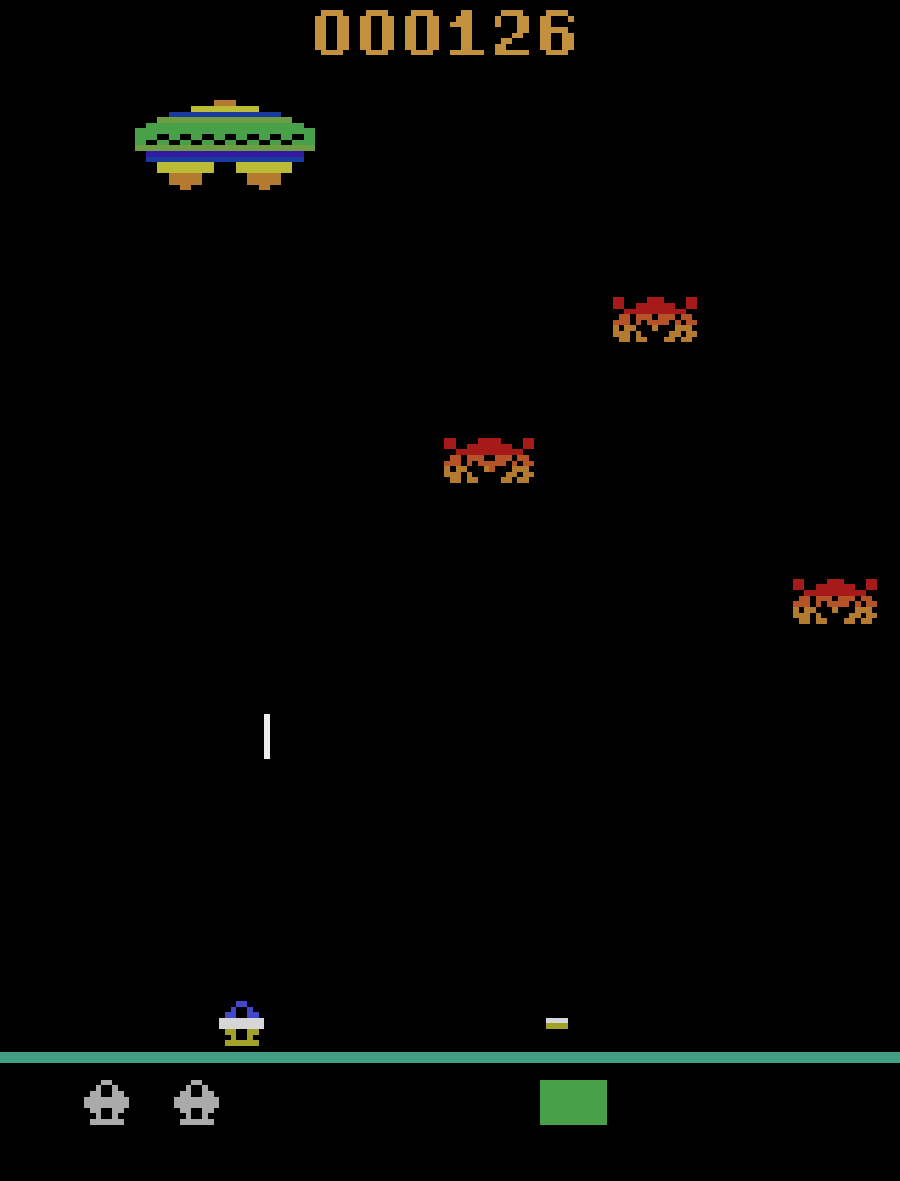
\includegraphics[width=0.3\linewidth]{img/assault_preview.png}
    \caption{Atari Assault environment.}
    \label{fig:assault_preview}
\end{figure}

For our modular framework, we break the objective down to a multi-objective problem, where each alien ship is viewed as a separate objective, and each local policy attempts to destroy its assigned target while avoiding enemy missiles. 
Not only does this facilitate an improvement in the performance, as we will demonstrate, but also we obtain a transparent design, because which target is being chased is revealed at each point. 
This modular design is made possible by the object-centric variant of the Atari environment \citep{delfosse2023ocatari}, which exposes the states of each individual target and the missiles by decoding the RAM states. 
The full observation space of each local policy also include the current position of the missile launcher, the current health, and the number of remaining lives. 
The local policy gets a reward or a penalty upon destroying its target enemy ship or losing a life, respectively. 
For local policy $i$, the Assault reward is
\[
    r_i =
    r_i^{\mathrm{destroy}}
    + r_i^{\mathrm{life}}
    + r_i^{\mathrm{overheat}}
    + r_i^{\mathrm{hot}}
    + r_i^{\mathrm{bid}}
    + r_i^{\mathrm{window}} .
\]
The destroy reward is credited to the policy assigned to the destroyed enemy, while life-loss, overheat, and fire-while-hot penalties discourage unsafe firing behavior.
The bid and action-window terms account for the auction mechanism.
Lastly, we use the game score as the metric for evaluation.
The Assault environment parameters are listed in~\Cref{tab:assault-env-params}, and the corresponding multi-policy, single-policy PPO, and DWN training parameters are listed in~\Cref{tab:assault-mappo-hparams,tab:assault-ppo-hparams,tab:assault-dwn-hparams}.

\textbf{Environment III: Atari Air-Raid.} Air-Raid uses the same modular Atari setup: each incoming enemy is treated as an objective and assigned to a local policy.
Positive score changes are interpreted as enemy kills, and each kill yields a destroy reward proportional to the score increase.
We also penalize near misses from enemy missiles: if an enemy missile enters a fixed box around the player without causing a life loss, the controlling policy receives a near-hit penalty.
For local policy $i$, the Air-Raid reward is
\[
    r_i =
    r_i^{\mathrm{destroy}}
    + r_i^{\mathrm{near\text{-}hit}}
    + r_i^{\mathrm{bid}} .
\]
Destroy rewards are credited to the policy associated with the hit enemy when that policy owns the player missile that caused the score event, near-hit penalties are assigned to the policy currently controlling the player, and bid penalties are applied according to the auction rule.
The single-policy PPO baseline uses the destroy and near-hit terms without bid penalties.
Additional training and implementation details are reported in~\Cref{sec:reprod-details}.


\textbf{Baseline approaches.}
We compare our method against two baselines: a single policy PPO with weighted rewards and deep W-learning (DWN; \citep{rosero2024multi}). 
For the PPO baseline, since all objectives have the same importance across the environments, we use the total reward across objectives at each step as the reward function.
We note that in Atari Assault, the single-policy PPO reward includes enemy-destroy rewards, raw score rewards, life-loss penalties, overheat penalties, and fire-while-hot penalties, but no bid or action-window terms.
The observation space remains the same as the multi-policy setting. 
In the Cat Feeder environment, we implement three reward mechanisms to help guide learning: one only with the sparse rewards from the environment, one with distance-based dense reward with respect to the nearest feeding request (denoted Nearest Shaping/NS in the experiments), and finally one where we provide distance-based reward with respect to the request that has the least amount of time until expiration (denoted Expiry Shaping/ES).
The PPO implementation is taken from CleanRL~\citep{huang2022cleanrl}.
We use the specified PPO hyperparameters from CleanRL for the Atari games and we tune the hyperparameters for the Cat Feeder environment with 40 Optuna iterations~\citep{akiba2019optuna}.

DWN is another multi-policy method for multi-objective RL that uses DQN for each of the local policies and additionally learns a W-network for each policy that predict scalar weights. 
These weights are used to choose which policy's action should be played at each step. 
The W-network is trained alongside the Q-network by updating it with a gradient step to predict the negative temporal difference (TD) error when the policy does not get to play its action.
The assertion here is that the negative TD-error quantifies how important it is for the policy to play its action. 
The implementation is borrowed from the repository of \citep{rosero2024multi}. All hyperparameters for the baselines are listed in~\Cref{sec:reprod-details}.
